\documentclass[11pt]{article}

\usepackage{fullpage}
\usepackage{tikz}
\usetikzlibrary{shapes.geometric, arrows}
\tikzstyle{startstop} = [rectangle, rounded corners, minimum height=0.5cm,text centered, draw=black, fill=red!30]
\tikzstyle{io} = [trapezium, trapezium left angle=70, trapezium right angle=110, minimum height=0.5cm, text centered, draw=black, fill=blue!30]
\tikzstyle{process} = [rectangle, minimum width=3cm, minimum height=1cm, text centered, draw=black, fill=orange!30]
\tikzstyle{decision} = [diamond, minimum width=1cm, minimum height=1cm, text centered, draw=black, fill=green!30]
\tikzstyle{arrow} = [thick,->,>=stealth]    

\begin{document}

\title{ARM Checkpoint report}
\author{Fawwaz Abdullah (ws420), Robert Buxton (rb419), \\Edward Hartley (ech120), Wojtek Sowinski (ws420) }

\maketitle

\section{Group Organisation}

\subsection{Work Distribution and Coordination}

In our initial group meeting, we planned out how we wanted to first approach 
creating the emulator. We decided to initially work together on designing the 
data types and structures, and then implemented the decoder and the overarching 
fetch-execute cycle. \\ \\
After this was completed, we distributed the four categories
of instruction between the team members. Fawwaz worked on branch, Robert on data
processing, Edward on the single data transfer and Wojtek on multiply. After
code was committed it was reviewed by other teammates. Once all the subsections were complete we worked together as a team to fix bugs
and remove redundancies in the code. 

\subsection{Evaluation and Future Strategies}

Our primary method of communication is Discord where we have a video meeting at 
11 am every day to discuss how the project is going and where we plan to go next.
We also communicate frequently in the chat which means that the team has a good
idea of the state of the project and any problems can be resolved promptly. \\ \\
What we would like to do in the future is find ways to reduce the amount of 
downtime when team is waiting for bottlenecks to be completed. We think we can 
achieve this by spending more time planning before starting on the next section.

\section{Implementation}

\subsection{Emulator Data Structures}

\begin{itemize}

    \item \textbf{Program State} (\texttt{State}): A struct representing the 
    processor's current state. It holds the current fetched and 
    decoded flags, a pointer to an array of values representing 
    all of the registers excluding the CPSR, A pointer to an array of values 
    representing the processors memory, The next instruction to be decoded, the 
    next instruction to be executed, 
    the CPSR register and lastly the last accessed memory address.
    
    \item \textbf{Decoded instruction} (\texttt{Instruction}): A struct representing
    a decoded instruction. It holds a condition code, a type referring to which 
    instruction it is and lastly a strut representing the specific instruction be executed.
    
    \item \textbf{Instruction types} There are 5 instruction types, data processing,
    multiply, single data transfer, branch and halt and they all have a strut
    representing them containing all the required data to execute them

    
    \end{itemize}

\subsection{Emulator Program Structure}

\begin{itemize}
    \item \texttt{decoder.c} Decodes raw binary into one of the 5 instruction 
    types.
    \item \texttt{branch.c} Simulates the branch instruction.
    \item \texttt{dataprocessing.c} Simulates one the ten data processing 
    instructions.
    \item \texttt{halt.c} Halts the program.
    \item \texttt{multiply.c} Simulates the multiply instruction.
    \item \texttt{singledatatransfer.c} Simulates single data transfer instructions.
    \item \texttt{fetcher.c} Fetches the next instruction from memory and
    increments the PC.
    \item \texttt{emulate.c} initializes the processor and starts the fetch decode
    execute cycle on the binary file provided. 
    \item \texttt{printstate.c} Prints the final state of the program after 
    halting.
\end{itemize}

\subsection{Emulator Program Flow}

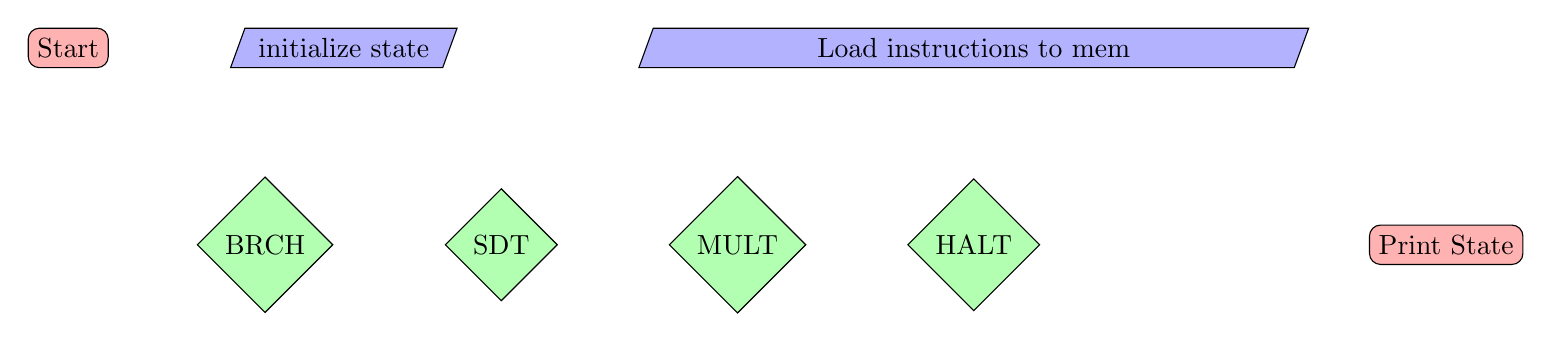
\begin{tikzpicture}[node distance=2cm]
    \node (start) [startstop] {Start};
    \node (in1) [io, right of=start, xshift=1.5cm] {initialize state};
    \node (in2) [io, right of=in1, xshift=6cm, inner sep=0] {Load instructions to mem};
    \node (dec1) [decision, below of=in2, yshift=-0.5cm] {HALT};
    \node (start) [startstop, right of=dec1, xshift=4cm] {Print State};
    \node (dec2) [decision, left of=dec1, xshift = -1cm] {MULT};
    \node (dec3) [decision, left of=dec2, xshift = -1cm] {SDT};
    \node (dec4) [decision, left of=dec3, xshift = -1cm] {BRCH};
    
\end{tikzpicture}

\subsection{Future Tasks}


\end{document}
